\chapter{Results}


\section{Numerical results}
In this chapter we present the results of the numerical experiments, where we have implemented the finite volume method for solving the shallow water equations in 1D and tested it on several problems.
\footnote{Code and small animations can be found at github, visit \url{https://github.com/MelissaJessen/Shallow-Water-Equations}.}
A key focus is to verify the implementation, as it will be used to generate data for the data-driven methods, including neural networks and Fourier neural operators.

\subsection{The 1D Dam Break Problem}
First we solve the 1D dam break problem, with the following initial conditions:
\begin{align*}
    h(x,0) &= \begin{cases}
        h_L, & \text{if } x < x_0, \\
        h_R, & \text{if } x > x_0,
    \end{cases} 
\end{align*}
where $x \in [0, 50], h_L = 3.5$ m, $h_R = 1.25$ m and $x_0 = 20$ m.
Since it is a dam break problem the initial fluid velocity is zero, i.e., $u(x,0) = 0$.
We solve the problem starting at $t=0$ and ending at $t=2.5$ seconds.
The numerical solution to the 1D Dam Break Problem using the FVM, together with the true solution, provided from the course~\cite{phd_corse_2009}, can be seen in \autoref{fig:1D_dam_break}.
\begin{figure}[H]
    \centering
    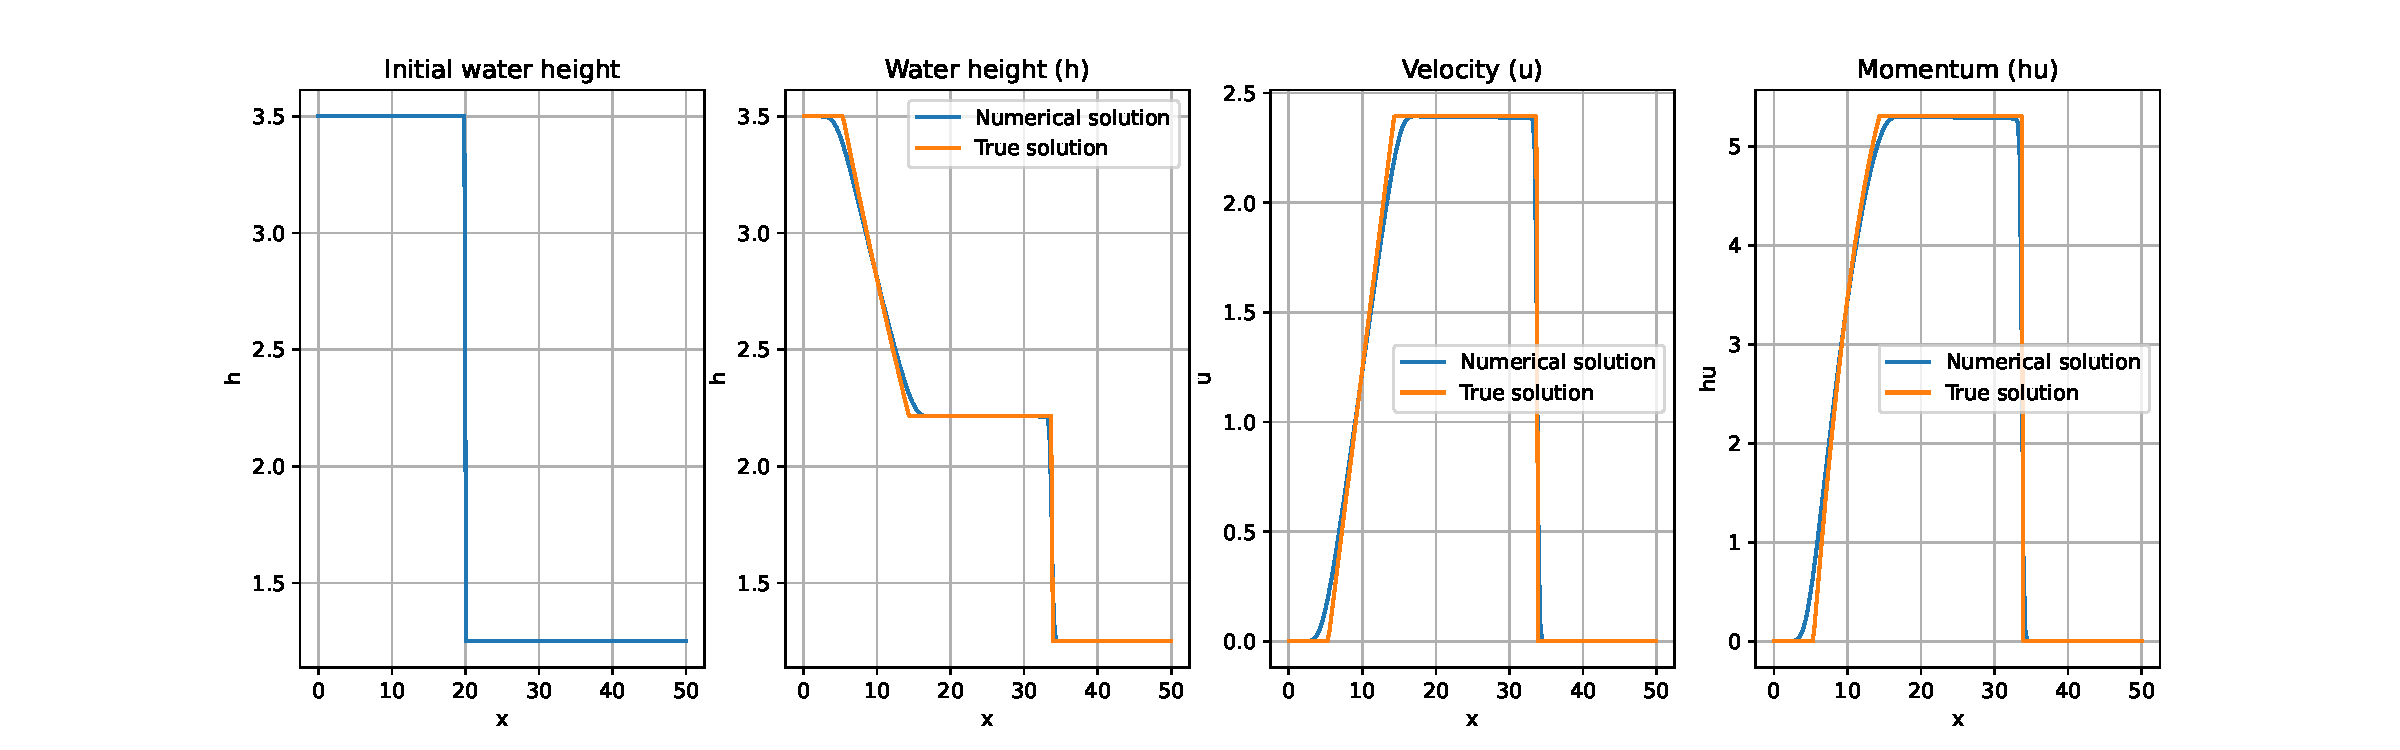
\includegraphics[width=0.95\textwidth]{C:/Users/Matteo/Shallow-Water-Equations/plots/sol_1D_val.pdf}
    \caption{The initial water height $h$ at $t=0$, together with the water height, the fluid velocity $u$ and the momentum $hu$ after $t=2.5$ seconds.}\label{fig:1D_dam_break}
\end{figure}
From Figure~\ref{fig:1D_dam_break} we see that the numerical solution aligns well with the true solution, and successfully captures the discontinuity.


\subsection{Toro test cases}
We have tested the method on the five test cases from Toros book~\cite{Toro2001-Shock}.
The initial conditions for the five test cases are given in \autoref{tab:toro_test_cases}.
\begin{table}[H]
    \centering
    \begin{tabular}{c|c|c|c|c|c|c}
        \hline
        \textbf{Test case} & \textbf{$h_L$} & \textbf{$u_L$} & \textbf{$h_R$} & \textbf{$u_R$} & \textbf{$x_0$} & \textbf{$t_{end}$} \\
        \hline\hline
        1 & 1.0 & 2.5 & 0.1 & 0.0 & 10.0 & 7.0 \\
        2 & 1.0 & -5.0 & 1.0 & 5.0 & 25.0 & 2.5 \\
        3 & 1.0 & 0.0 & 0.0 & 0.0 & 20.0 & 4.0 \\
        4 & 0.0 & 0.0 & 1.0 & 0.0 & 30.0 & 4.0 \\
        5 & 0.1 & -3.0 & 0.1 & 3.0 & 25.0 & 5.0 \\
        \hline
    \end{tabular}
    \caption{Initial conditions for the five test cases.}\label{tab:toro_test_cases}
\end{table}
The domain is $x \in [0, 50]$ for all test cases.
The test cases are chosen to test the method on different types of waves, such as shock waves and rarefaction waves.
To solve the test cases there are used different fluxes, namely:
\begin{enumerate}
    \item Godunov method with exact Riemann solver,
    \item Lax-Friedrich flux,
    \item Lax-Wendroff flux,
    \item FORCE flux,
    \item HLL flux,
\end{enumerate}

\subsubsection*{Test case 1}
%\addcontentsline{toc}{subsection}{Test case 1}
The initial conditions for test case 1 are given in \autoref{fig:toro_test1_initial} and the final solution after $t=7.0$ seconds is given in \autoref{fig:toro_test1_final}.
In test case 1, we observe a right shock wave and a left rarefaction wave.
\begin{figure}[H]
    \centering
    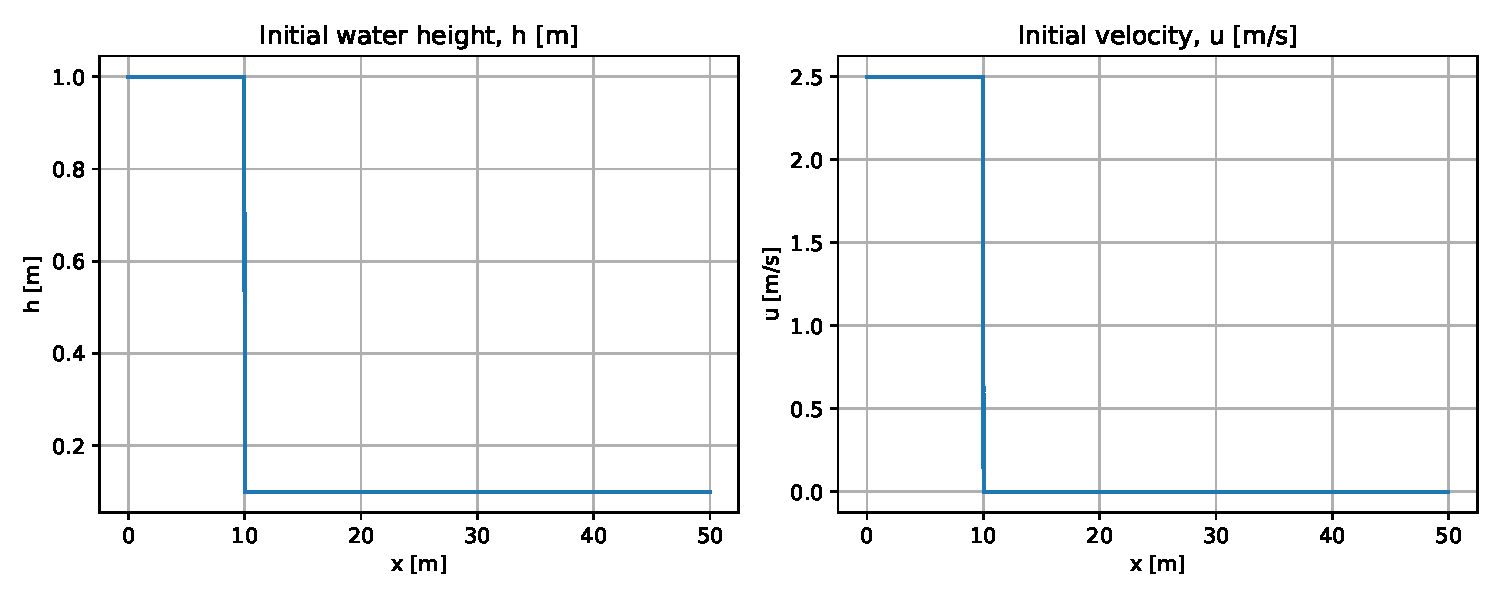
\includegraphics[width=0.7\textwidth]{C:/Users/Matteo/Shallow-Water-Equations/plots/toro_test1_initial.pdf}
    \caption{Initial conditions for the test case.}\label{fig:toro_test1_initial}
\end{figure}

\begin{figure}[H]
    \centering
    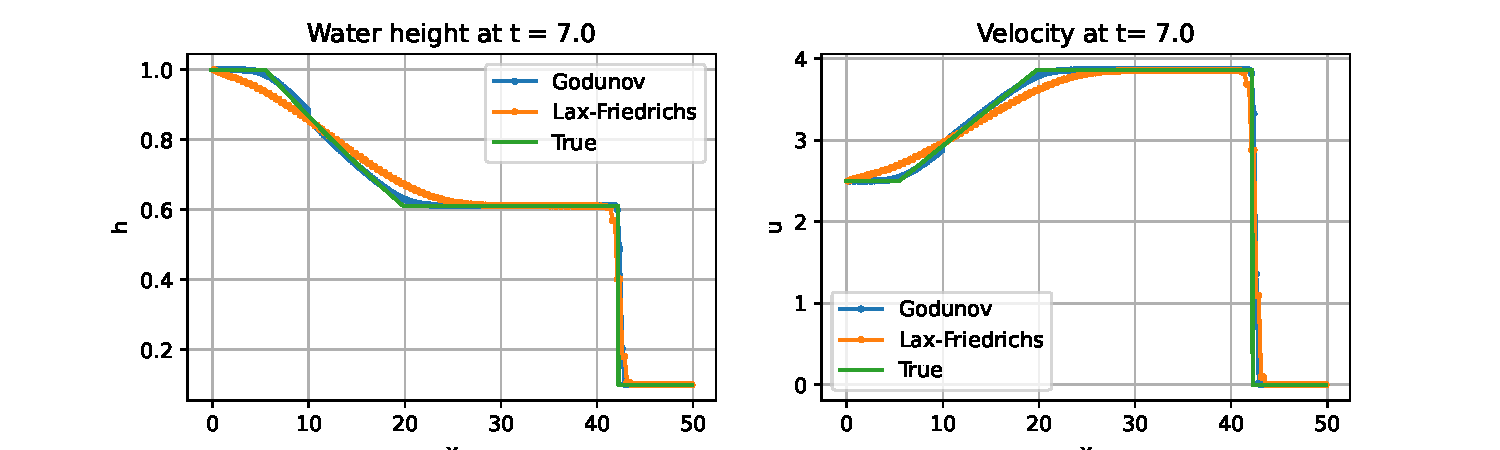
\includegraphics[width=0.7\textwidth]{C:/Users/Matteo/Shallow-Water-Equations/plots/toro_test1_final.pdf}
    \caption{Final solution for the test case.}\label{fig:toro_test1_final}
\end{figure}
For this test case all the fluxes work well, but there are minor differences in the solution, which can be seen in \autoref{fig:toro_test1_final}.

\subsubsection*{Test case 2}
%\addcontentsline{toc}{subsection}{Test case 2}
The initial conditions for test case 2 are illustrated in \autoref{fig:toro_test2_initial}.
\begin{figure}[H]
    \centering
    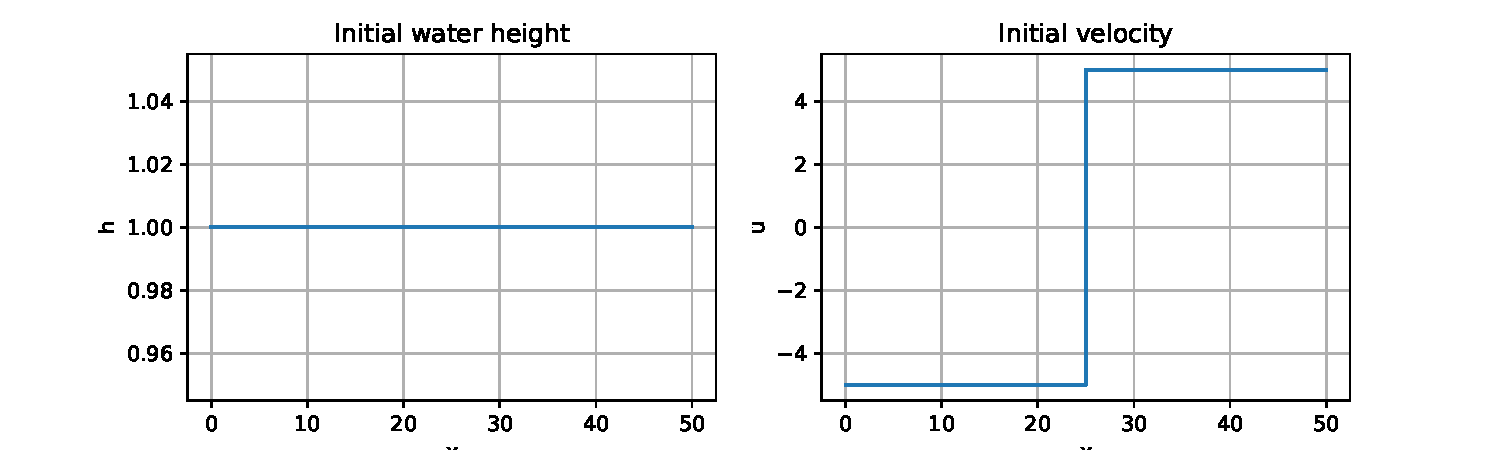
\includegraphics[width=0.7\textwidth]{C:/Users/Matteo/Shallow-Water-Equations/plots/toro_test2_initial.pdf}
    \caption{Initial conditions for the test case.}\label{fig:toro_test2_initial}
\end{figure}
In test case 2 we have two rarefaction waves, one on the left side and one on the right side.
As they are travelling in opposite directions (away from each other), there will be created a nearly dry bed in the middle of the domain.
Many methods have difficulties with this test case as they may compute a negative water height.
For these experiments we were able to get close to the true solution, using Lax-Friedrich flux, FORCE flux and HLLC flux.
The final solution after $t=2.5$ seconds is given in \autoref{fig:toro_test2_final}.

\begin{figure}[H]
    \centering
    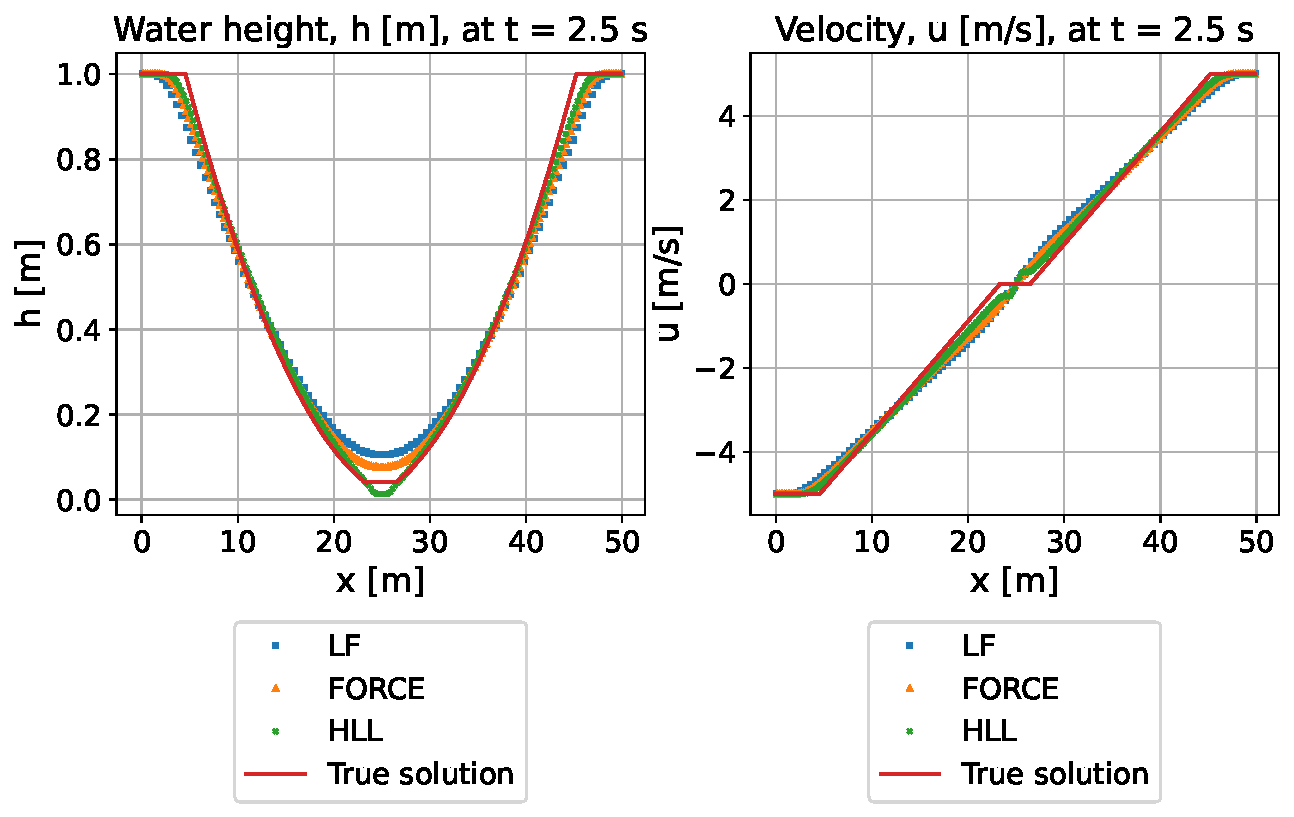
\includegraphics[width=0.7\textwidth]{C:/Users/Matteo/Shallow-Water-Equations/plots/toro_test2_final.pdf}
    \caption{Final solution for the test case.}\label{fig:toro_test2_final}
\end{figure}
For some of the other fluxes, Godunov method with exact Riemann solver, Lax-Wendroff or flux-splitting/upwind, it was not possible to get an acceptable solution.

\subsubsection*{Test case 3}
%\addcontentsline{toc}{subsection}{Test case 3}
The initial conditions for test case 3 are given in \autoref{fig:toro_test3_initial}, and the final solution after $t=4.0$ seconds is given in \autoref{fig:toro_test3_final}.
\begin{figure}[H]
    \centering
    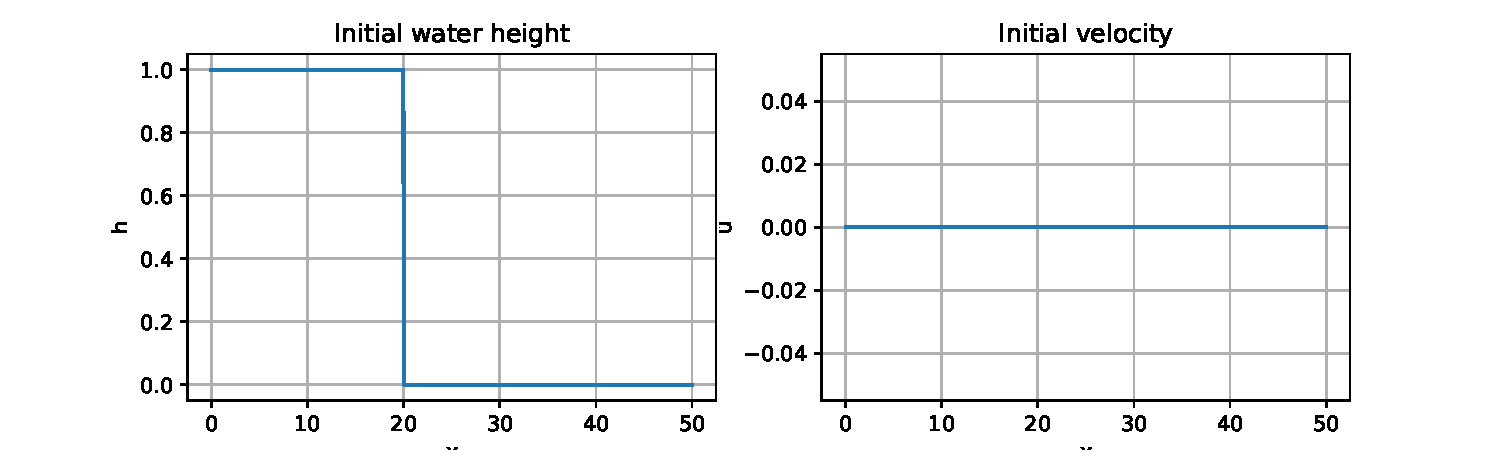
\includegraphics[width=0.7\textwidth]{C:/Users/Matteo/Shallow-Water-Equations/plots/toro_test3_initial.pdf}
    \caption{Initial conditions for the test case.}\label{fig:toro_test3_initial}
\end{figure}

\begin{figure}[H]
    \centering
    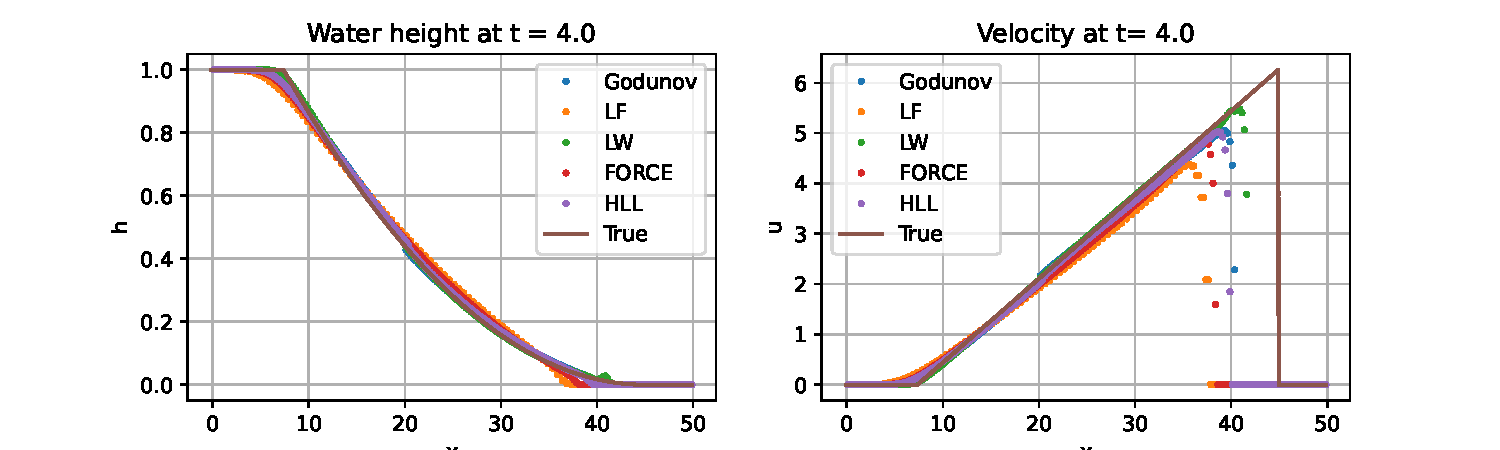
\includegraphics[width=0.7\textwidth]{C:/Users/Matteo/Shallow-Water-Equations/plots/toro_test3_final.pdf}
    \caption{Final solution for the test case.}\label{fig:toro_test3_final}
\end{figure}
To solve case 3, with the FVM we must add a small amount to $h_R$, since the code does not handle $h_R = 0$ well.
We set $h_R = 0.00005$ to solve it numerically, but the true solution is for $h_R = 0$.
By running experiments with different values of $h_R$, we see that the solution converges to the true solution as $h_R$ approaches 0.
The solution consists of a left rarefaction wave.

\subsubsection*{Test case 4}
%\addcontentsline{toc}{subsection}{Test case 4}
The initial conditions for test case 4 are given in \autoref{fig:toro_test4_initial}, and the final solution after $t=4.0$ seconds is given in \autoref{fig:toro_test4_final}.
\begin{figure}[H]
    \centering
    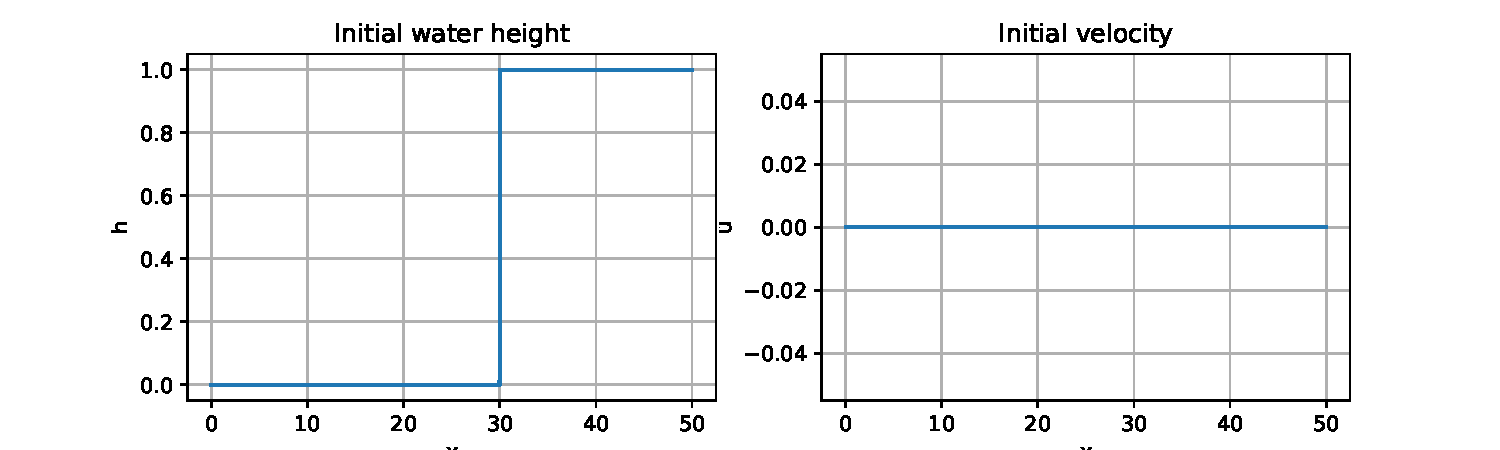
\includegraphics[width=0.7\textwidth]{C:/Users/Matteo/Shallow-Water-Equations/plots/toro_test4_initial.pdf}
    \caption{Initial conditions for the test case.}\label{fig:toro_test4_initial}
\end{figure}

\begin{figure}[H]
    \centering
    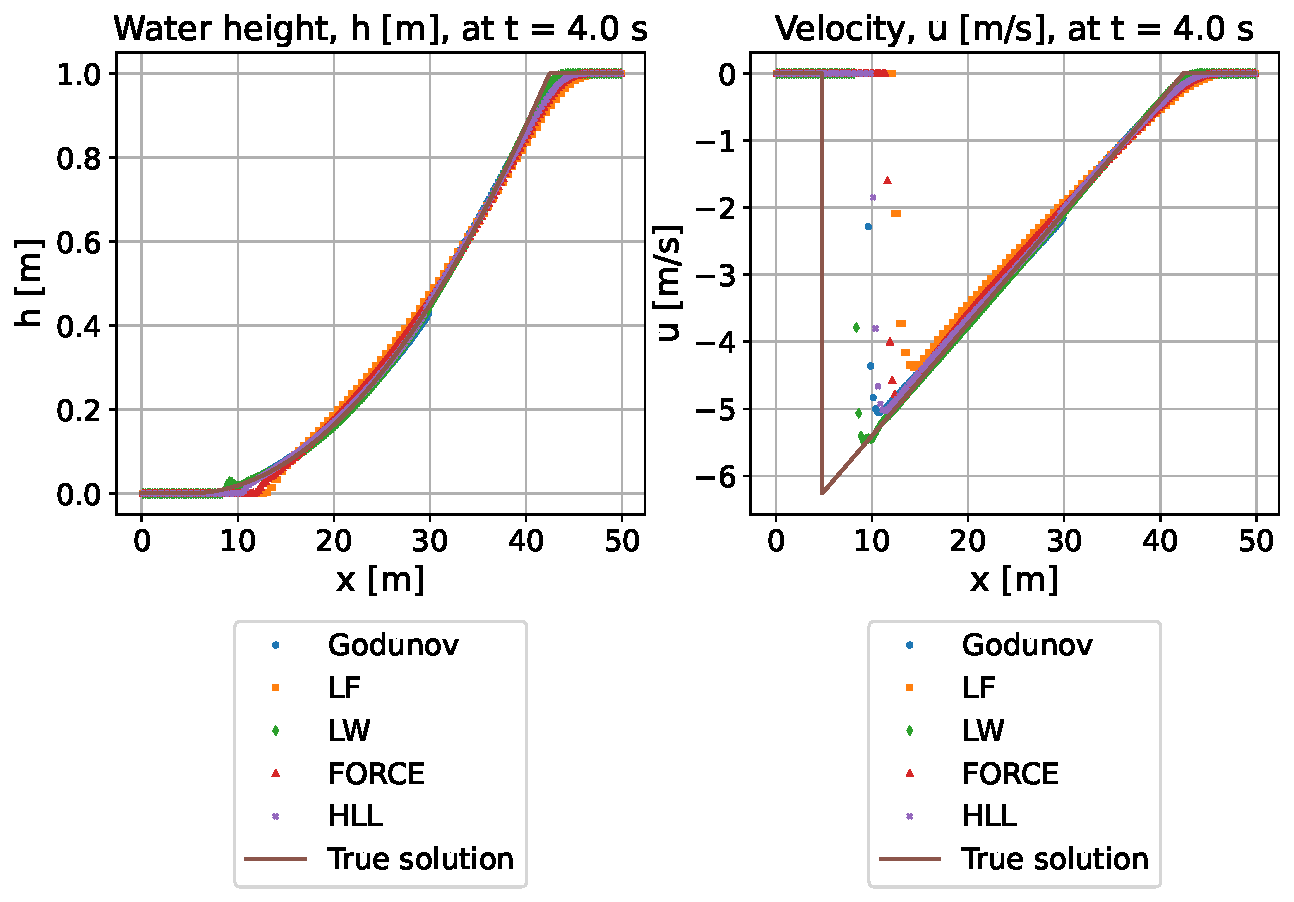
\includegraphics[width=0.7\textwidth]{C:/Users/Matteo/Shallow-Water-Equations/plots/toro_test4_final.pdf}
    \caption{Final solution for the test case.}\label{fig:toro_test4_final}
\end{figure}
In case 4 we face the same challenges as in case 3.
We set $h_L = 0.00005$, and the solution converges to the true solution as $h_L$ approaches 0.
This test case is symmetric to test case 3, and the solution consists of a right rarefaction wave.
The case is included to test if the results are as expected.

\subsubsection*{Test case 5}
%\addcontentsline{toc}{subsection}{Test case 5}
The initial conditions for test case 5 are given in \autoref{fig:toro_test5_initial}, and the final solution after $t=5.0$ seconds is given in \autoref{fig:toro_test5_final}.
\begin{figure}[H]
    \centering
    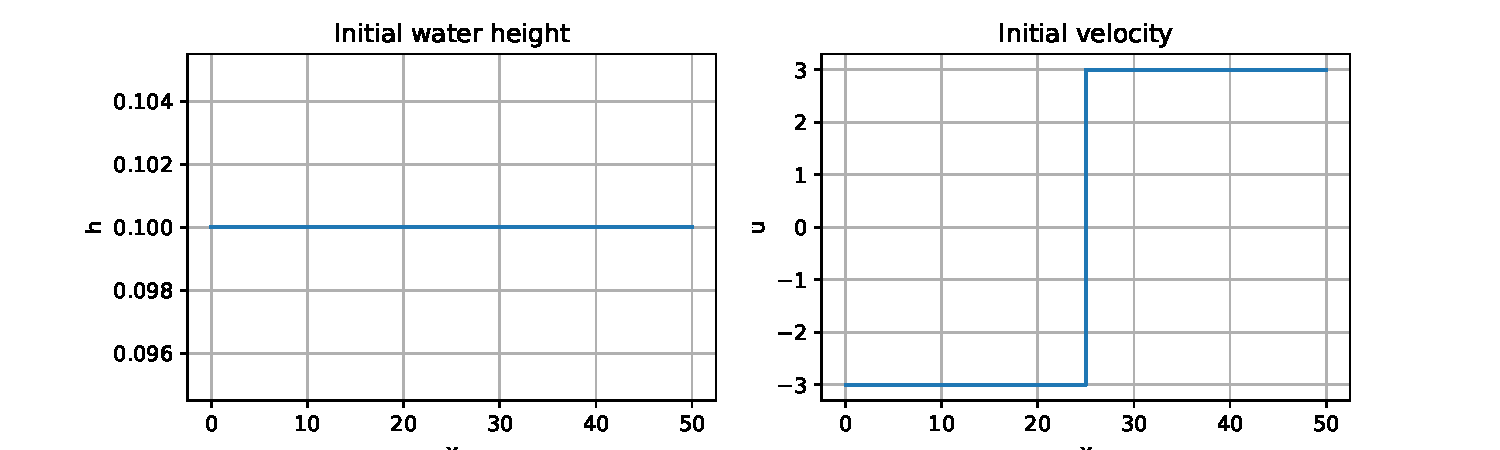
\includegraphics[width=0.7\textwidth]{C:/Users/Matteo/Shallow-Water-Equations/plots/toro_test5_initial.pdf}
    \caption{Initial conditions for the test case.}\label{fig:toro_test5_initial}
\end{figure}

\begin{figure}[H]
    \centering
    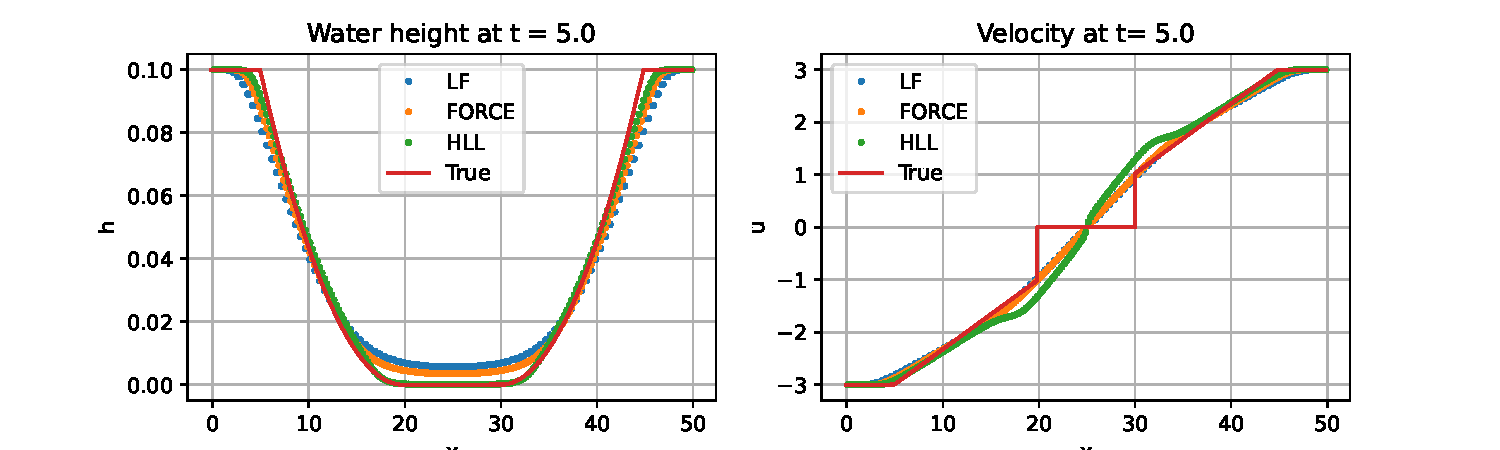
\includegraphics[width=0.7\textwidth]{C:/Users/Matteo/Shallow-Water-Equations/plots/toro_test5_final.pdf}
    \caption{Final solution for the test case.}\label{fig:toro_test5_final}
\end{figure}
From~\autoref{fig:toro_test5_final} we see that the numerical solutions for the velocity $v$ at $t=5.0$ are smooth, where the true solution is discontinuous. 
In this test case there are also challenges with some of the fluxes due to the generation of a dry-bed region.
The fluxes that dont work are: Godunov method with exact RP, Lax-Wendroff and flux-splitting/upwind.
The solution consists of two rarefaction waves, one on the left side and one on the right side, and a dry-bed region in the middle.

To get an overview of which fluxes that were able to solve the problems, consider the table below.

\begin{table}[H]
    \centering
    \begin{tabular}{c|c|c|c|c|c}
        \hline
        \textbf{Test case} & \textbf{Godunov} & \textbf{LF} & \textbf{LW} & \textbf{FORCE} & \textbf{HLL}   \\
        \hline\hline
        1 & $\checkmark$ & $\checkmark$ & $\checkmark$ & $\checkmark$ & $\checkmark$   \\
        2 & $\times$ & $\checkmark$ & $\times$ & $\checkmark$ & $\checkmark$ \\
        3 & $\checkmark$ & $\checkmark$ & $\checkmark$ & $\checkmark$ & $\checkmark$  \\
        4 & $\checkmark$ & $\checkmark$ & $\checkmark$ & $\checkmark$ & $\checkmark$  \\
        5 & $\times$ & $\checkmark$ & $\times$ & $\checkmark$ & $\checkmark$  \\
        \hline
    \end{tabular}
    \caption{Overview of which fluxes that were able to solve the test cases.}
    \label{tab:toro_fluxes}
\end{table}



\subsection{2D idealised Circular Dam Break Problem}
Consider the idealised circular dam break problem with a horizontal bottom.
We assume there is an infinitely thin circular wall at radius $R = 2.5$ m is a square domain of size $40 \times 40 $ with centre at $(x_c,y_c) = (20, 20)$.
The initial conditions are (ch. 15 Toro)
\begin{align*}
    h(x,y,0) &= \begin{cases}
        2.5 \text{ }m, & \text{if } \sqrt{ {(x-x_c)}^2 + {(y-y_c)}^2 } \leq R, \\
        0.5 \text{ }m, & \text{otherwise},
    \end{cases} \\
    u(x,y,0) &= 0, \\
    v(x,y,0) &= 0.
\end{align*}
%Use the WAF method (chapter 11) along with a second-order dimensional splitting scheme (chapter 12).
%CFL-condition: $C_{cfl} = 0.9$.
%van Leer limiter. Mesh: $200 \times 200$.
We use a mesh of size $200 \times 200$.
The results after $t=0.0, 0.4, 0.7$ and $1.4$ seconds are given in \autoref{fig:2D_dam_break_grid}.
\begin{figure}[H]
    \centering
    \begin{subfigure}{0.49\textwidth}
        \centering
        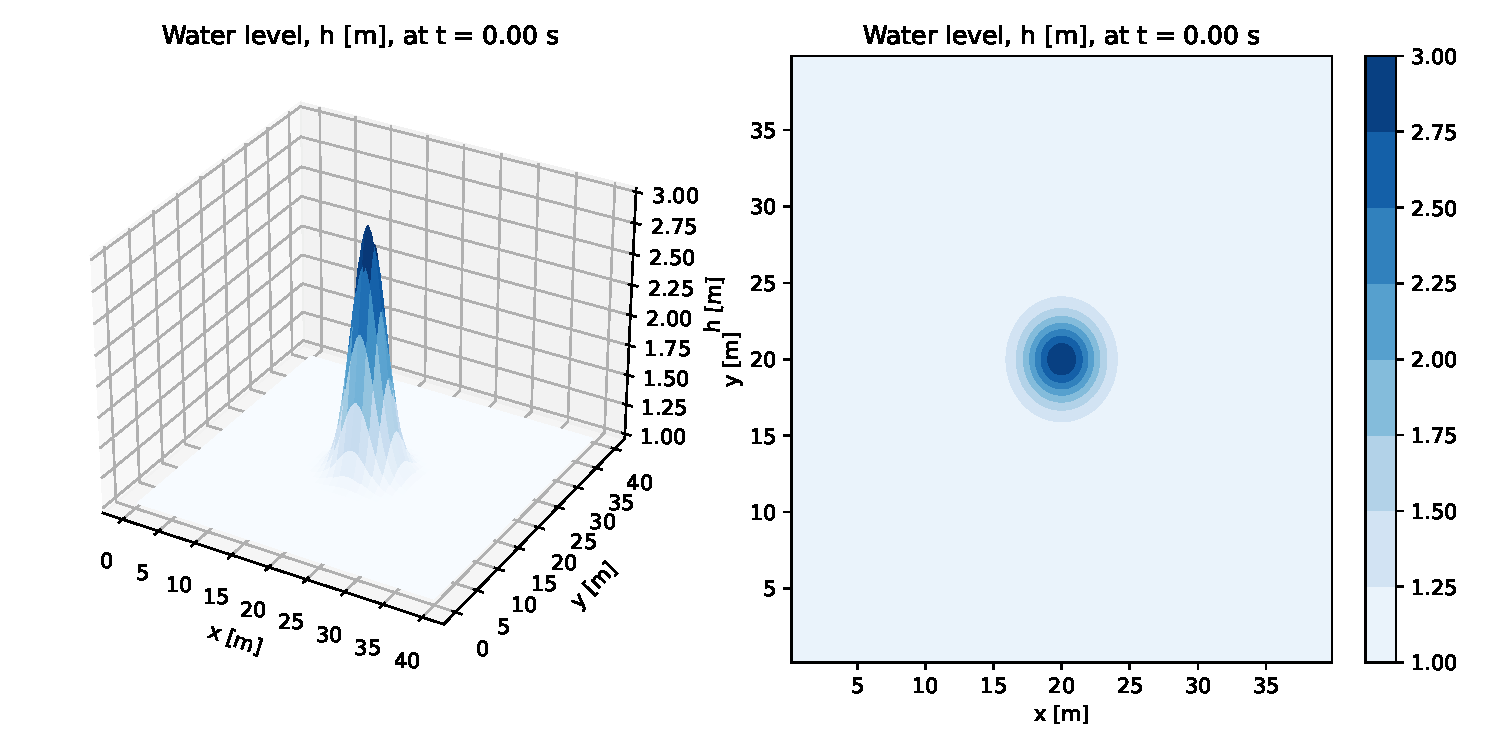
\includegraphics[width=\textwidth]{C:/Users/Matteo/Shallow-Water-Equations/plots/toro2D_t=0.pdf}
        \caption{2D dam break problem after $t=0$.}\label{fig:2D_dam_break_t0}
    \end{subfigure}
    \hfill
    \begin{subfigure}{0.49\textwidth}
        \centering
        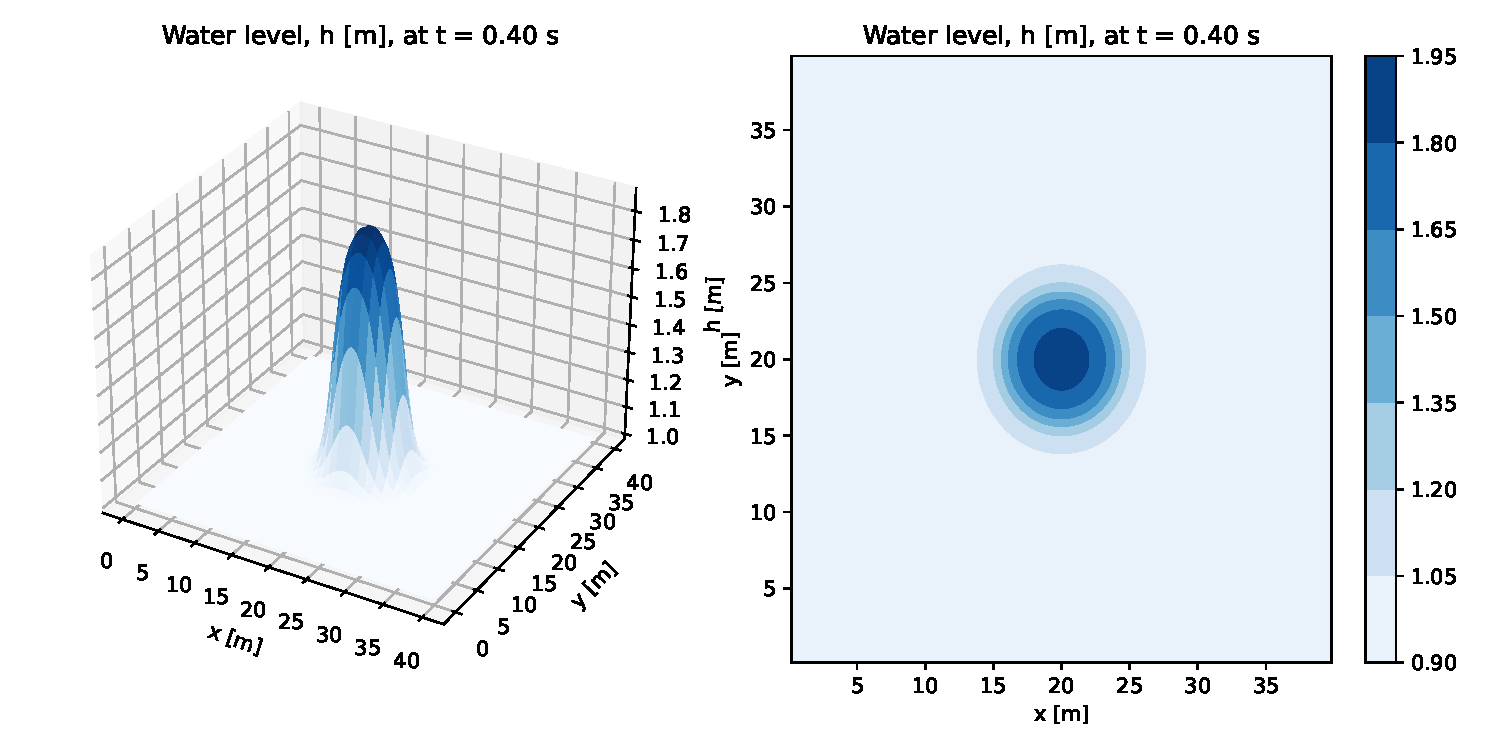
\includegraphics[width=\textwidth]{C:/Users/Matteo/Shallow-Water-Equations/plots/toro2D_t=0.4.pdf}
        \caption{2D dam break problem after $t=0.4$.}\label{fig:2D_dam_break_t0.4}
    \end{subfigure}

    \vspace{0.5cm} % Adjusts vertical space between rows

    \begin{subfigure}{0.49\textwidth}
        \centering
        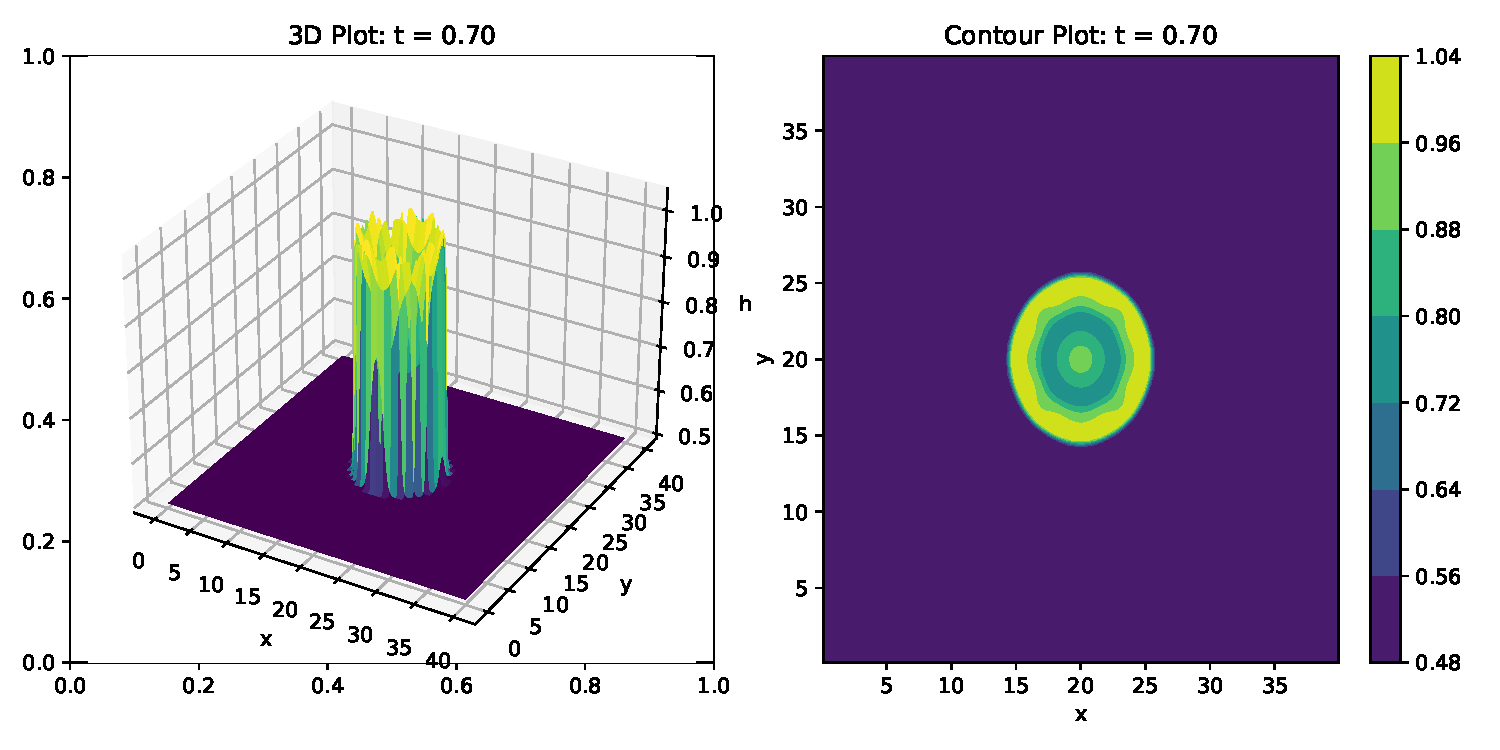
\includegraphics[width=\textwidth]{C:/Users/Matteo/Shallow-Water-Equations/plots/toro2D_t=0.7.pdf}
        \caption{2D dam break problem after $t=0.7$.}\label{fig:2D_dam_break_t0.7}
    \end{subfigure}
    \hfill
    \begin{subfigure}{0.49\textwidth}
        \centering
        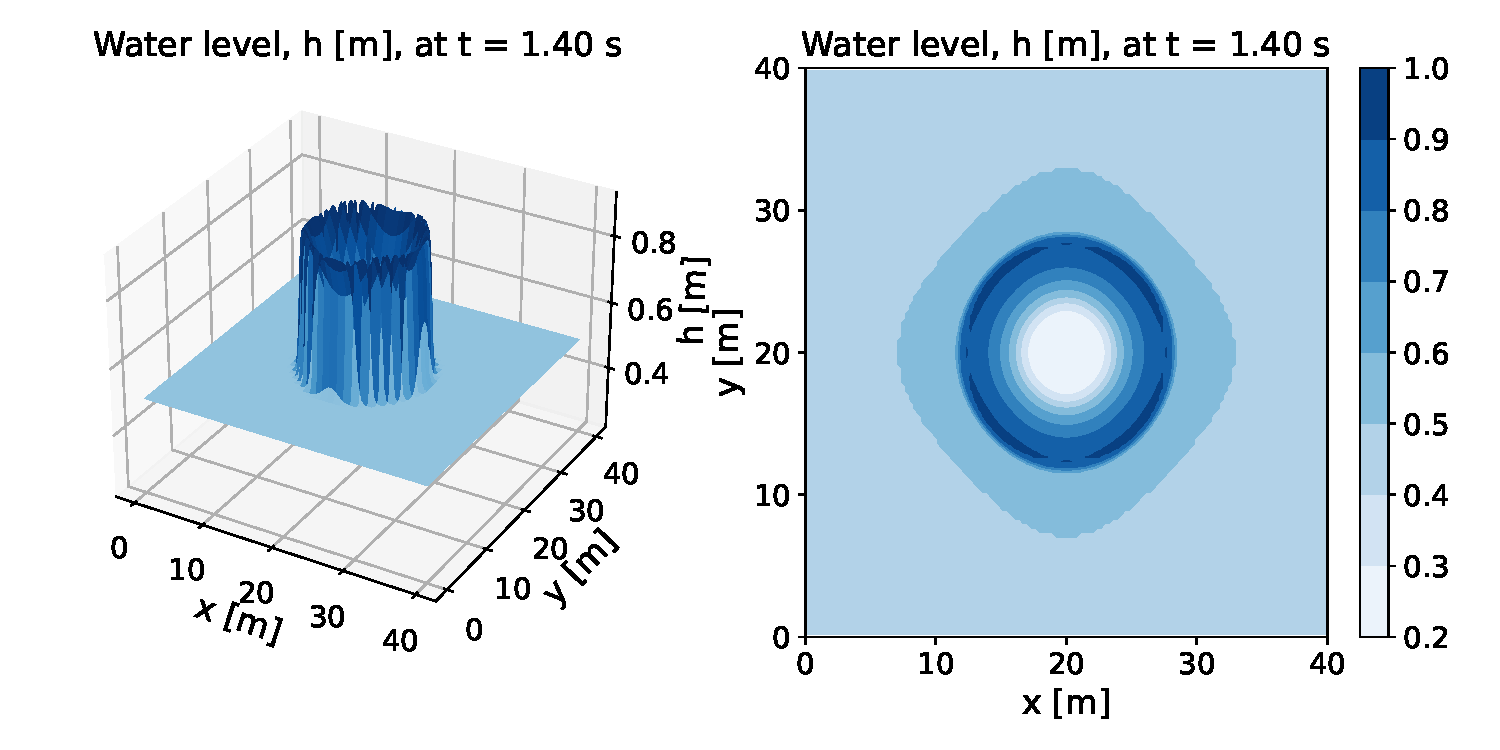
\includegraphics[width=\textwidth]{C:/Users/Matteo/Shallow-Water-Equations/plots/toro2D_t=1.4.pdf}
        \caption{2D dam break problem after $t=1.4$.}\label{fig:2D_dam_break_t1.4}
    \end{subfigure}

    \caption{Snapshots of the 2D dam break problem at different times.}\label{fig:2D_dam_break_grid}
\end{figure}

By comparing \autoref{fig:2D_dam_break_grid} with the results from the book by Toro~\cite{Toro2024}, and see that the numerical solution aligns well with the true solution from the book.





